\documentclass{beamer}
\usetheme{default}
\usepackage{graphicx}
\usepackage{hyperref}
\usepackage{amsmath}
\usepackage{listings}

\lstdefinelanguage{GLSL}
{
sensitive=true,
morekeywords=[1]{
attribute, const, uniform, varying,
layout, centroid, flat, smooth,
noperspective, break, continue, do,
for, while, switch, case, default, if,
else, in, out, inout, float, int, void,
bool, true, false, invariant, discard,
return, mat2, mat3, mat4, mat2x2, mat2x3,
mat2x4, mat3x2, mat3x3, mat3x4, mat4x2,
mat4x3, mat4x4, vec2, vec3, vec4, ivec2,
ivec3, ivec4, bvec2, bvec3, bvec4, uint,
uvec2, uvec3, uvec4, lowp, mediump, highp,
precision, sampler1D, sampler2D, sampler3D,
samplerCube, sampler1DShadow,
sampler2DShadow, samplerCubeShadow,
sampler1DArray, sampler2DArray,
sampler1DArrayShadow, sampler2DArrayShadow,
isampler1D, isampler2D, isampler3D,
isamplerCube, isampler1DArray,
isampler2DArray, usampler1D, usampler2D,
usampler3D, usamplerCube, usampler1DArray,
usampler2DArray, sampler2DRect,
sampler2DRectShadow, isampler2DRect,
usampler2DRect, samplerBuffer,
isamplerBuffer, usamplerBuffer, sampler2DMS,
isampler2DMS, usampler2DMS,
sampler2DMSArray, isampler2DMSArray,
usampler2DMSArray, struct},
morekeywords=[2]{
radians,degrees,sin,cos,tan,asin,acos,atan,
atan,sinh,cosh,tanh,asinh,acosh,atanh,pow,
exp,log,exp2,log2,sqrt,inversesqrt,abs,sign,
floor,trunc,round,roundEven,ceil,fract,mod,modf,
min,max,clamp,mix,step,smoothstep,isnan,isinf,
floatBitsToInt,floatBitsToUint,intBitsToFloat,
uintBitsToFloat,length,distance,dot,cross,
normalize,faceforward,reflect,refract,
matrixCompMult,outerProduct,transpose,
determinant,inverse,lessThan,lessThanEqual,
greaterThan,greaterThanEqual,equal,notEqual,
any,all,not,textureSize,texture,textureProj,
textureLod,textureOffset,texelFetch,
texelFetchOffset,textureProjOffset,
textureLodOffset,textureProjLod,
textureProjLodOffset,textureGrad,
textureGradOffset,textureProjGrad,
textureProjGradOffset,texture1D,texture1DProj,
texture1DProjLod,texture2D,texture2DProj,
texture2DLod,texture2DProjLod,texture3D,
texture3DProj,texture3DLod,texture3DProjLod,
textureCube,textureCubeLod,shadow1D,shadow2D,
shadow1DProj,shadow2DProj,shadow1DLod,
shadow2DLod,shadow1DProjLod,shadow2DProjLod,
dFdx,dFdy,fwidth,noise1,noise2,noise3,noise4,
EmitVertex,EndPrimitive},
morekeywords=[3]{
gl_VertexID,gl_InstanceID,gl_Position,
gl_PointSize,gl_ClipDistance,gl_PerVertex,
gl_Layer,gl_ClipVertex,gl_FragCoord,
gl_FrontFacing,gl_ClipDistance,gl_FragColor,
gl_FragData,gl_MaxDrawBuffers,gl_FragDepth,
gl_PointCoord,gl_PrimitiveID,
gl_MaxVertexAttribs,gl_MaxVertexUniformComponents,
gl_MaxVaryingFloats,gl_MaxVaryingComponents,
gl_MaxVertexOutputComponents,
gl_MaxGeometryInputComponents,
gl_MaxGeometryOutputComponents,
gl_MaxFragmentInputComponents,
gl_MaxVertexTextureImageUnits,
gl_MaxCombinedTextureImageUnits,
gl_MaxTextureImageUnits,
gl_MaxFragmentUniformComponents,
gl_MaxDrawBuffers,gl_MaxClipDistances,
gl_MaxGeometryTextureImageUnits,
gl_MaxGeometryOutputVertices,
gl_MaxGeometryOutputVertices,
gl_MaxGeometryTotalOutputComponents,
gl_MaxGeometryUniformComponents,
gl_MaxGeometryVaryingComponents,gl_DepthRange},
morecomment=[l]{//},
morecomment=[s]{/*}{*/},
morecomment=[l][keywordstyle4]{\#},
}

\lstset{
backgroundcolor=\color[rgb]{0.95, 0.95, 0.95},
tabsize=2,
rulecolor=,
basicstyle=\scriptsize,
upquote=true,
aboveskip={1.5\baselineskip},
columns=fixed,
showstringspaces=false,
extendedchars=true,
breaklines=true,
prebreak = \raisebox{0ex}[0ex][0ex]{\ensuremath{\hookleftarrow}},
frame=single,
showtabs=false,
showspaces=false,
showstringspaces=false,
identifierstyle=\ttfamily,
keywordstyle=\color[rgb]{1.0,0,0},
keywordstyle=[1]\color[rgb]{0,0,0.75},
keywordstyle=[2]\color[rgb]{0.5,0.0,0.0},
keywordstyle=[3]\color[rgb]{0.127,0.427,0.514},
keywordstyle=[4]\color[rgb]{0.4,0.4,0.4},
commentstyle=\color[rgb]{0.133,0.545,0.133},
stringstyle=\color[rgb]{0.639,0.082,0.082},
}
\title{
    Fluid Simulation with\\
    Smoothed Particle Hydrodynamics(SPH) method\\
    accelerated with Compute Shaders\\
    ${\quad}$\\
    \small{Final project for the practical course in Computergrafik 2016}
}
\author{Fabian Klemp\\
    \small{FH Aachen}\\
}
\date{30 June, 2016}
\setbeamertemplate{bibliography item}{}
\setbeamertemplate{footline}{\hspace*{\fill}\insertframenumber/\inserttotalframenumber\hspace*{\fill}\vskip15pt}
\usenavigationsymbolstemplate{}
\begin{document}
{
\setbeamertemplate{footline}{}
\begin{frame}[noframenumbering]
    \maketitle
\end{frame}
}
\begin{frame}
    \frametitle{Table of Contents}
    \tableofcontents
\end{frame}

\section{Introduction}
\begin{frame}
    \frametitle{Fluids}
    \begin{itemize}
        \item Liquids, e.g. water
        \item Gasses, e.g. air
        \item Plasmas
    \end{itemize}
\end{frame}
\begin{frame}
    \frametitle{Motivation}
    \begin{center}
        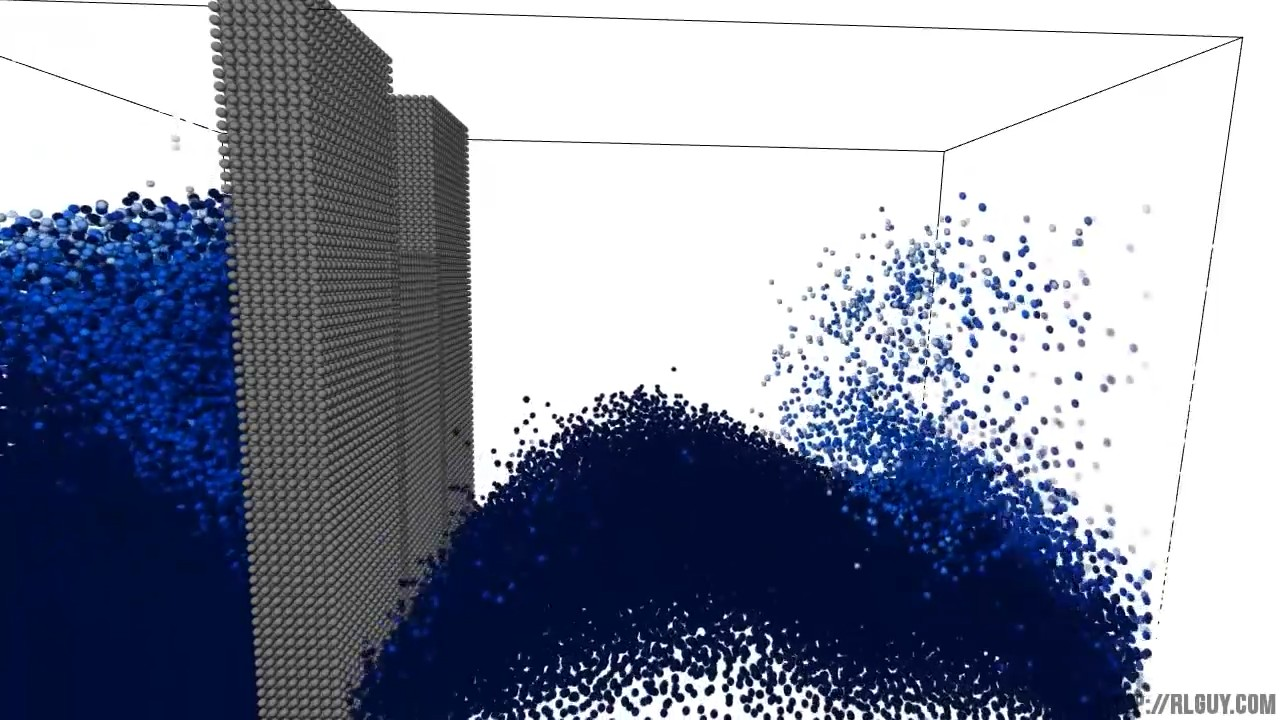
\includegraphics[width=10cm]{introduction.jpg}
    \end{center}
    \begin{flushright}
        source: \href{https://youtu.be/iHACAlfYeiQ}{youtu.be/iHACAlfYeiQ}
    \end{flushright}
\end{frame}


\section{Formula}
\begin{frame}
    \frametitle{Navier-Stokes-Equations}
    Equations which describe the motion of viscous fluids.\\
    $\qquad$\\
    We use the Navier-Stokes-Equations for incompressible fluids with constant density:\\
    \begin{align*}
        \frac{\partial\boldsymbol{v}}{\partial t} + (\boldsymbol{v} \cdot \nabla )\boldsymbol{v} = 
        \boldsymbol{g} - \nabla \frac{\boldsymbol{p}}{\rho} + \frac{\mu}{\rho}\nabla^2\boldsymbol{v} 
    \end{align*}
    where $\boldsymbol{v}$ is the velocity, $\boldsymbol{g}$ is the gravity,
    $\boldsymbol{p}$ is the pressure and $\rho$ and $\mu$ are the material
    properties density and dynamic viscosity.
\end{frame}

\begin{frame}
    \frametitle{Smoothed Particle Hydrodynamics}
    Physical property $\Phi_i$ at position $r_i$ is computed in a sphere with radius $h$:
    \begin{align*}
        \Phi_i = \sum_j m_j W(h, \boldsymbol{r_i} - \boldsymbol{r_j})
    \end{align*}
    $W$ is the weighting function which sums to $1$ over radius $h$ and drops to $0$ outside of $h$.
\end{frame}

\begin{frame}
    \frametitle{Smoothed Particle Hydrodynamics}
    \begin{align*}
        \rho_i &\approx \sum_j m_j \frac{315}{64\pi h^9} \big(h^2-\lVert \boldsymbol{r_i} - \boldsymbol{r_j} \rVert^2\big)^3\\
        %
        p_i &= \rho_i - \rho_0\\
        %
        \frac{\nabla\boldsymbol{p_i}}{\rho_i} &\approx \sum_j m_j \bigg( \frac{\boldsymbol{p_i}}{\rho_i^2} + \frac{\boldsymbol{p_j}}{\rho_j^2}\bigg) 
        \frac{-45}{\pi h^6} \big(h-\lVert\boldsymbol{r_i} - \boldsymbol{r_j}\rVert\big) \frac{\boldsymbol{r_i} - \boldsymbol{r_j}}{\lVert \boldsymbol{r_i} - \boldsymbol{r_j}\rVert}\\
        %
        \frac{\mu}{\rho_i}\nabla^2\boldsymbol{v_i} &\approx \frac{\mu}{\rho_i}\sum_j m_j \bigg(\frac{\boldsymbol{v_j} - \boldsymbol{v_i}}{\rho_j}\bigg)
        \frac{45}{\pi h^6}\big(h - \lVert\boldsymbol{r_i} - \boldsymbol{r_j}\rVert\big)\\
        %
        \frac{dv_i}{dt} &= \boldsymbol{g} -  \frac{\nabla\boldsymbol{p_i}}{\rho_i} + \frac{\mu}{\rho_i}\nabla^2\boldsymbol{v_i}
    \end{align*}
\end{frame}

\section{Compute Shader}

\begin{frame}
    \frametitle{Compute Shader}
    \begin{itemize}
        \item Introduced with OpenGL 4.3
        \item Written in GLSL
        \item Can directly interface with other OpenGL buffers\\
            contrary to OpenCL, CUDA, etc.
        \item Run asynchronous per default
        \item Meant for simpler computational tasks
    \end{itemize}
\end{frame}

\begin{frame}
    \frametitle{Compute Shader Example}
    \lstinputlisting[language=GLSL]{wave.cmp}
\end{frame}

\begin{frame}
    \frametitle{Compute Shader Example}
    Use:
    \lstinputlisting[language=C++]{invoke.cpp}
\end{frame}

\section{Implementation}
\begin{frame}
    \frametitle{Concrete Implementation}
    \begin{itemize}
        \item Sort particles in voxel of length $h$
        \item Limit interaction with neighbour particles 
            \begin{itemize}
                \item Only interact with $n$ particles
                \item Only interact with particles within the interaction radius $h$
                \item Do this while preventing bias
            \end{itemize}
    \end{itemize}
\end{frame}

\begin{frame}
    \frametitle{Concrete Implementation}
    Compute Shaders:
    \begin{itemize}
        \item voxelize\\ $\quad$ calculate voxel id for each particle
        \item <2->sort\\ $\quad$ sort by voxel id
        \item <3->sortPostPass\\$\quad$rewrite position and velocity data
        \item <4->voxelIndex\\$\quad$calculate index from voxels to particles
        \item <5->findNeighbours\\$\quad$find the next $n$ neighbours in neighbouring voxels
        \item <6->computeDensityPressure\\$\quad$compute density and pressure values for each particles
        \item <7->integrate\\$\quad$compute pressure gradient, viscosity term, acceleration,\\$\quad$integrate velocity and position
    \end{itemize}
\end{frame}
\begin{frame}
    \frametitle{Concrete Implementation}
    A few words about findNeighbours:
    \begin{itemize}
        \item Search in each of the neighbouring voxels until $n$ neighbours within the interaction radius are found
        \item Compute random offset into voxel for each shader invocation then proceed sequentially
        \item Alternate searching direction by evenness of particle id
    \end{itemize}
\end{frame}

\section{Demo}
\begin{frame}
    \frametitle{Demo}
    \begin{center}
        Video/Demo
    \end{center}
\end{frame}
    
\begin{frame}
    \frametitle{Main problem}
    \begin{center}
        \visible<2->{I am a computer scientist not a physicist.\\$\quad$\\}
        \visible<3->{The algorithms work(AFAIK) but the numerics are shit.}
    \end{center}
\end{frame}

\section{Lessons learned}
\begin{frame}
    \frametitle{Lessons learned}
    \begin{itemize}
        \item Be sure to know your domain. Otherwise get an expert
        \item Before trying to accelerate something on the GPU implement it on the CPU
            \begin{itemize}
                \item Debugging is much easier/possible
                \item Easier to get working(more built-ins, more libs, etc.)
                \item Verification of performance and correctness
            \end{itemize}
        \item Be sure to do you research properly. Turns out nobody really uses this method anymore
    \end{itemize}
\end{frame}

\begin{frame}
    \frametitle{Appendix}
    Source code:
    \begin{center}
        \href{https://github.com/Faerbit/sphfluidsim}{github.com/Faerbit/sphfluidsim}
    \end{center}
    Source and implementation ideas:
    \begin{center}
        "Smoothed Particle Hydrodynamics" OpenCL Programming Webinar Series by AMD (November 29, 2010)\\
        \href{https://youtu.be/SQPCXzqH610}{Screencast} \href{http://developer.amd.com/wordpress/media/2012/10/SmoothedParticleHydrodynamics.pdf}{Slides}
    \end{center}
\end{frame}

\begin{frame}
    \frametitle{Thank you for your attention}
    \begin{center}
        Any Questions?\\
        Feedback?
    \end{center}
    
\end{frame}

\end{document}
